\documentclass[a4paper,10pt]{article}
\usepackage[utf8]{inputenc}
\usepackage[T1]{fontenc}
\usepackage[french]{babel}
\frenchbsetup{StandardLists=true} % à inclure si on utilise \usepackage[french]{babel}
\usepackage{enumitem}
\usepackage{amssymb}
\usepackage{graphicx}
\usepackage[gen]{eurosym}

% Title Page
\title{Rapport gestion de l'hotel}
\author{
  Romain PEREIRA\\
  \newline
  Douha OURIMI\\
  \and
  Laurie PANDRAUD\\
  \newline
  Yi LU\\
}
\date{Dimanche 10 Décembre 2017}

\usepackage{hyperref}
\hypersetup{
    colorlinks,
    citecolor=black,
    filecolor=black,
    linkcolor=blue,
    urlcolor=black
}


\begin{document}
\maketitle
\tableofcontents
  \section{Préambule}
    Autrefois dis 'le Bien-heureux', notre équipe a repris en main la gestion du nouvel hôtel 'Ocre'. La précèdente équipe l'a laissé dans un état négligé.
    Nous avons géré l'hôtel pendant ces 4 dernières années, et avons construit un modèle économiquement viable.
    \newline
    \newline
    L’hôtel Ocre s’établit dans un contexte de concurrence avec 6 autres établissements qui partent d’une situation économique similaire.
    L’hôtel a initialement une capacité d’accueil de 50 chambres qui ont été gérées par 4 employés permanents et 2 employés temporaires.
    Nous avons recuperé l'hotel en basse saison.
    \newline
    \newline
    De manière global, nous avons accordé une grande attention aux conditions de marchés, et à l'étude de nos résultats.
    La prise en compte des variations de la demande en fonction de la saison
    (été -haute saison, hiver - basse saison) et des acteurs extérieurs nous ont permis d’évaluer
    au mieux les besoins des clients, et de pouvoir ciblés les marchés. (nos estimations se sont souvent avérés très précises)
  \newpage
  \section{Stratégie de developpement : domestique}
    \subsection{Tour 1 : 1er hiver}      
      Dans un premier temps, la stratégie développée a été de faire de l’hotel Ocre un hotêl 'low cost',
      des prix attrayants, avec une rénovation à 87\%, pour s’accaparer une très grande part de marché.
      
      
    \subsection{Tour 2 - Tour 3}
      Cependant, nous avons remarqué que nos concurrents se dirigeait tous, sans exception, vers cette politique.
      C'est pourquoi, dés le 1er été, nous avons décidé de nous diriger vers du luxe,
      que ce soit au niveau de la qualité de la prestation ou du prix de la nuité.
      \newline
      \newline
      Nous comptions alors augmenter progressivement nos prix, au fur et à mesure que la demande de prestation de luxe augmente.
      Ainsi nous nous dirigeons sur le long terme, vers un autre type de marché et un autre type de clientèle.
      L’hôtel est rénové à plus de 95\% et l'inverstissement en formation des employés est augmenté pour une meilleure qualité de service.
      On augmente donc en proportion les salaires de nos employés.
      \newline
      \newline
      Nous decidons également d'investir (+ 50 000 \euro{} Figure \ref{effort_reduction_couts}) dans la reduction des coûts de maintenance et d'administration,
      car un hôtel de meilleur qualité implique de plus important frais de gestion, et nous comptons retombez sur cette investissement.
      \newline
      \newline
      Ce remaniement de l'hôtel nous a donc donné un 2ème hiver difficile, avec le plus mauvais chiffre d'affaire du secteur,
      mais nous savions que ce risque allait s'avérer rentable par la suite.

    \subsection{Tour 4 - Tour 8}
      Aussi,  l’investissement est nécessaire pour garder une dynamique de développement de l’hôtel. Avec une dette de 72\% de nos capitaux propres,
      nous decidons de l'augmenter à 80\% (soit 500 000 \euro{} d'emprunt) afin de construire 5 nouvelles chambres.
      \newline
      \newline
      Néanmoins, certains de nos concurrents (O'Tel et No Name) ont décidé de nous concurrencer sur le luxe.
      Ils ont augmenter la qualité des prestations de leur hôtel.
      C’est pourquoi notre stratégie s’est orienté des prestations de qualités, à prix bon marché.
      Avec des marges plus faible, on assure tout même une bonne rentabilité de notre établissement,
      augmentons notre part de marché, et diminuons celle de nos concurrents. (voir Tour 4 Figure \ref{remplissage_hotel})
      \newline
      \newline
      Ayant 1 année d'avance, nous essayons de rester les plus compétitifs pour les prochains tours, en étudiant les choix de nos concurrents.

      
   \newpage
   \section{Stratégie de developpement : international}
    
    \subsection{Tour 1 - Tour 2}
      Notre équipe a decidé de s'implanter à l'international dés le 1er tour.
      \newline
      Notre stratégie globale à long terme était de louer beaucoup de chambres, et peu chère. En s'assurant de faibles marges,
      sur les 1ères saisons, on esperait tuer la concurrence et obtenir le monopole du marché sur le long terme.
      \newline
      \newline
      Le 1er hiver, nous decidons donc de louer 20 chambres (le maximum possible) pour la prochaine haute saison.
      \newline
      \newline
      Arrivé à l'été, les conditions de marchés indiquent que la demande internationale a une bonne dynamique.
      Ayant recuperé les locaux dans un parfait état, et voyant que nos concurrents ont peu de chambres sur le marché international,
      nous optons pour une politique de prix élevés (~ 140 \euro{} / nuits), en esperant que l'offre sature par rapport à la demande.
      Notre politique de marketting est défensive: nous nous alignons sur nos concurrents, afin de limiter les frais.
      \newline
      Ces choix n'ont pas été efficace: nos locaux sont seulement occupés à 73\%, alors que nos concurrents retombent eux plus facilement sur les frais.
      Nous avons pris note de cette erreur et ajusterons nos prix pour les prochaines saisons.
      \newline
      \newline
      Convaincu par notre stratégie, nous prenons 10 chambres de plus, pour un total de 30 chambres pour le prochain hiver.
      \newline
      Les faibles résultats de cette saison hivernale s'explique par cette investissement.
    \subsection{Tour 3 - Tour 8}
      Le marché international ne connait finalement pas l'essor attendu. L'épisode de grippe aviaire au 2ème été a détruit le marché.
      (voir Figure \ref{ventes_internationales})
      Nous ne prenons donc pas de chambres supplémentaires, et rentabilisons au mieux nos chambres. (peu de renovations, optimisations des charges du personnels, maximum de préventes en agence).
      \newline
      En limitant ainsi les risques à l'international, nous concentrons nos investissements sur le marché domestique.
      \newline
      \newline
      Le marché reprends de la dynamique au dernier été. Grâce à notre politique de prix bas, nous obtenons la plus grosse part du marché, en se plaçant nettement devant
      'La Rose' 'Hotel Aviv', qui sont nos concurrents directes. Nous esperons ainsi les essoufler et croître plus vite qu'eux sur le long terme.

  \newpage
  \section{Perspectives futures et conclusion}

  Nous avons appliqué une stratégie que l’on pourrait qualifier d’adaptative.
  Finalement la dernière s’est révélée être la meilleure. Nous finissons le dernier tour
  avec 1 254 875 \euro{} de chiffre d’affaire, 372 795 \euro{} de cash en fin de saison.
  Notre ratio dette sur capitaux propres n’a pas beaucoup évolué car nous avons continué
  d’investir en achetant 10 nouvelles chambres. Cela explique l’augmentation de notre
  dette à long terme de 3 354 725 \euro{} à 3 755 725 \euro{}, ce qui ramène notre ratio
  dette sur capitaux propres à 82,70\%. L’augmentation rapide de la capacité de notre hôtel
  va permettre d’accueillir plus de clients et de prendre l’avantage sur nos concurrents.
  \newline
  \newline
  Notre hôtel a gagné en qualité, grâce à la rénovation à 100\%
  que nous avons effectuée et maintenue, mais aussi grâce au personnel
  très bien formé. Cela a permis au rapport qualité-prix de bien augmenter
  ce qui a attiré de nombreux clients.Le taux d’occupation domestique est désormais
  de 80,9\%, pour un résultat net par chambre de 3 031,57\euro{}.
  \newline
  \newline
  Nous avons progressé à l’international où nous n’étions pas présents.
  Notre taux d’occupation est actuellement de 92,1\%.
  Pour les saisons à venir, une rénovation complète de l’hôtel et une meilleure formation du personnel,
  pourrait permettre d’atteindre les 100\% de taux d’occupation de nos concurrents Sunrise et No Name. 
  \newline
  \newline
  La stratégie d’avoir le meilleur rapport qualité-prix a été très efficace.
  Cependant nos concurrents s’adaptent vite et commencent à nous imiter.
  Notamment O’Tel qui nous rattrappe actuellement et nous dépasse même
  sur le dernier été. Pour les saisons à venir, il sera donc important de s’adapter et de profiter
  de l’avantage que nous offre les dix chambres supplémentaires. Il sera important de faire plus de
  marketing pour attirer de nouveaux clients et d’augmenter la qualité de notre hôtel.


  \newpage
  \section{Graphiques, chiffres...}
    Ces quelques graphiques illustrent nos propos. Nous comparons ici nos données avec nos 2 principaux concurrents.
    \newline
        
    \begin{figure}[!ht]
      \begin{center}
	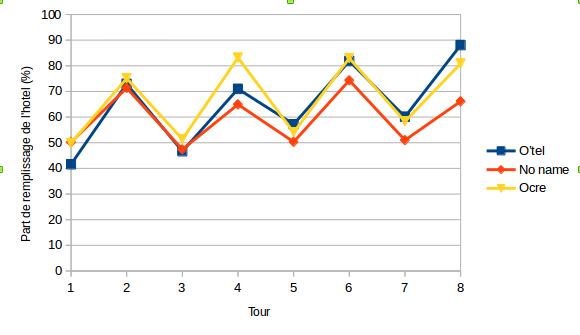
\includegraphics[height=7cm,keepaspectratio]{./images/remplissage_hotel.png}
      \end{center}
      \caption{\textit{Remplissage de l'hôtel (domestique)}}
      \label{remplissage_hotel}
    \end{figure}
    
    \begin{figure}[!ht]
      \begin{center}
	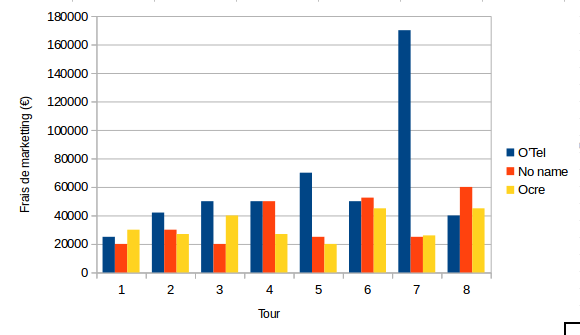
\includegraphics[height=7cm,keepaspectratio]{./images/frais_marketting.png}
      \end{center}
      \caption{\textit{Frais marketting}}
    \end{figure}
    
    \begin{figure}[!ht]
      \begin{center}
	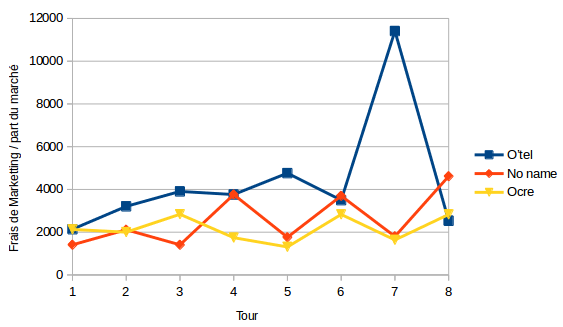
\includegraphics[height=7cm,keepaspectratio]{./images/marketting_part_marche.png}
      \end{center}
      \caption{\textit{Remplissage de l'hôtel en fonction des frais de marketting (domestique)}}
      \label{marketting_part_marche}
    \end{figure}
    
    \begin{figure}[!ht]
      \begin{center}
	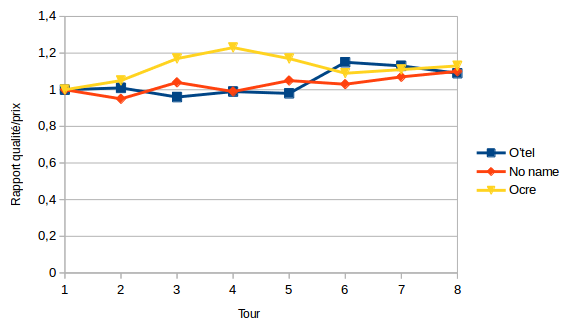
\includegraphics[height=7cm,keepaspectratio]{./images/rapport_qualite_prix.png}
      \end{center}
      \caption{\textit{Rapport qualité/prix (domestique)}}
    \end{figure}

    \begin{figure}[!ht]
      \begin{center}
	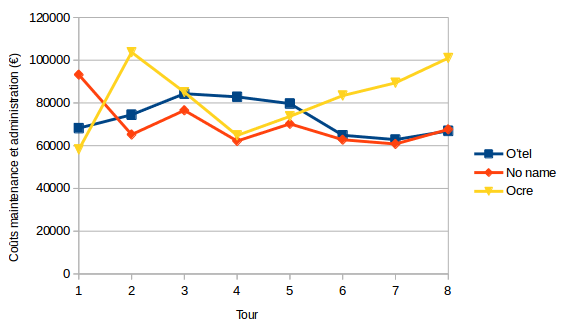
\includegraphics[height=7cm,keepaspectratio]{./images/cout_administration_et_maintenance.png}
      \end{center}
      \caption{\textit{Coût d'administration et de maintenance (domestique)}}
    \end{figure}

    
    \begin{figure}[!ht]
      \begin{center}
	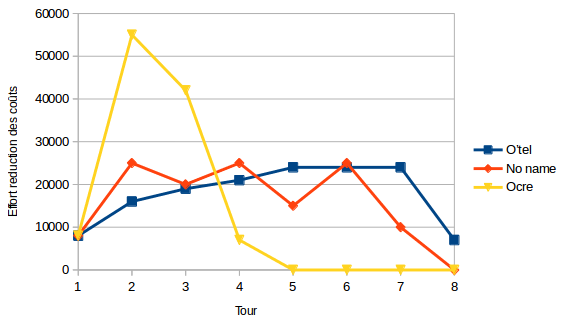
\includegraphics[height=7cm,keepaspectratio]{./images/effort_reduction_couts.png}
      \end{center}
      \caption{\textit{Effort reductions des coûts (domestique)}}
      \label{effort_reduction_couts}
    \end{figure}
    
    \begin{figure}[!ht]
      \begin{center}
	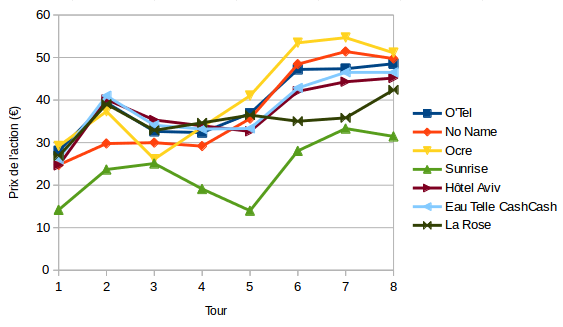
\includegraphics[height=7cm,keepaspectratio]{./images/action.png}
      \end{center}
      \caption{\textit{Prix de l'action}}
    \end{figure}
        
    \begin{figure}[!ht]
      \begin{center}
	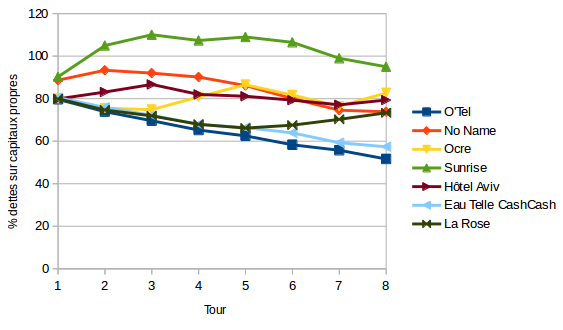
\includegraphics[height=7.0cm,keepaspectratio]{./images/dettes_capitaux.png}
      \end{center}
      \caption{\textit{Dettes sur capitaux propres (en \%)}}
    \end{figure}
    
    \begin{figure}[!ht]
      \begin{center}
	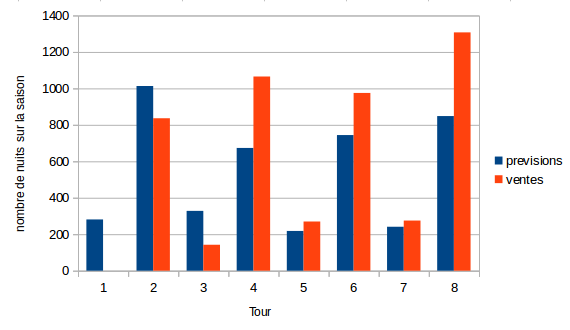
\includegraphics[height=7.0cm,keepaspectratio]{./images/ventes_internationales.png}
      \end{center}
      \caption{\textit{Nombre de nuits vendu au guichet par saison (international)}}
      \label{ventes_internationales}
    \end{figure}

\end{document}          
